\documentclass[twocolumn]{article}
\usepackage{graphicx}
\usepackage{hyperref}

% Generated by analysis/table_1_fit_results.ipynb -- do not edit by hand
\newcommand{\NGroups}{4}
\newcommand{\NPointsPerGroup}{11}
\newcommand{\SteepestGroup}{D}
\newcommand{\SteepestSlope}{$1.64 \pm 0.04$}
\newcommand{\MaxChiSqPerDof}{1.00}

\title{Example paper: releasing code and data alongside the text}
\author{Your Name\\Your Institute}
\date{\today}

\begin{document}

\maketitle

\begin{abstract}
A minimal paper showing figures, tables and quoted numbers that are all
generated by notebooks in the accompanying data release.
\end{abstract}

\section{Introduction}
Every figure, table and number in this paper is produced by a notebook in
the data release~\cite{data_release}. The code and small data products are
available at \url{https://YOUR_ORG.github.io/YOUR_REPO}.

\section{Results}
We fit a straight line to the \NPointsPerGroup{} measurements in each of
\NGroups{} groups. The steepest slope, \SteepestSlope, is found for
group~\SteepestGroup, and every fit has $\chi^2/\mathrm{dof} \leq
\MaxChiSqPerDof$. Figure~\ref{fig:measurements} shows the measurements and
fits, and Table~\ref{tab:fits} lists the fitted parameters.

\begin{figure}
    \centering
    % Generated by analysis/figure_1_measurements.ipynb
    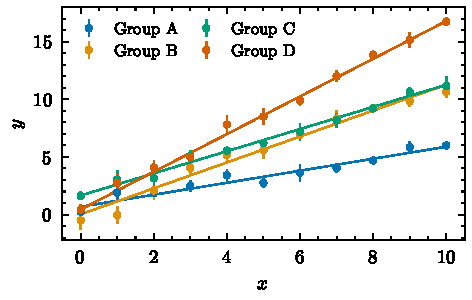
\includegraphics[width=\columnwidth]{figure_1_measurements.pdf}
    \caption{Measurements for each group, with the best-fit straight line.}
    \label{fig:measurements}
\end{figure}

\begin{table}
    \centering
    % Generated by analysis/table_1_fit_results.ipynb
    \begin{tabular}{c|cc|c}
    \hline
    Group & Slope & Intercept & $\chi^2/\mathrm{dof}$ \\
    \hline
    A & $0.52 \pm 0.04$ & $0.68 \pm 0.25$ & 1.00 \\
    B & $1.13 \pm 0.06$ & $0.02 \pm 0.38$ & 0.92 \\
    C & $0.96 \pm 0.04$ & $1.65 \pm 0.26$ & 0.41 \\
    D & $1.64 \pm 0.04$ & $0.44 \pm 0.28$ & 0.58 \\
    \hline
    \end{tabular}
    \caption{Best-fit slope and intercept, with $1\sigma$ uncertainties, and
    the reduced $\chi^2$ of the fit for each group.}
    \label{tab:fits}
\end{table}

\bibliographystyle{plain}
\bibliography{bibliography}

\end{document}
